% !TeX root = RJwrapper.tex
\title{\(\pkg{rfPermute}\): Estimation of Predictor Importance Significance in
Random Forest Models}
\author{by Frederick I. Archer}

\maketitle

\abstract{%
One of the strengths of the ensemble machine learning algorithm, Random
Forest, is its ability to estimate the relative importance of predictors
within classification and regression models. However, there is no method
for identifying which predictors are significantly more important than
what would be expected by random chance. I present the
\(\CRANpkg{rfPermute}\) package which is a wrapper for the commonly used
\(\CRANpkg{randomForest}\) package that produces permutation-based
estimates of predictor importance significance. The package also
includes utility functions for summarizing and visualizing Random Forest
model results.
}

\subsection{Introduction}\label{introduction}

Since its inception, the ensemble machine learning algorithm, Random
Forest \citep{RN266}, has been rapidly gaining popularity as a powerful
tool for classification and uncovering patterns in complex data sets.
Because it is non-parametric and produces internally-validated
classification models, it has been used in a wide variety of fields
\citep{RN126, RN128, RN268}, and has proven to be robust in performance
tests against other commonly used modelling algorithms \citep{RN125}.

The most common implementation of Random Forest is the
\(\CRANpkg{randomForest}\) package \citep{RN127}. This package allows
easy specification of both classification and regression models and
provides several useful functions for summarizing their results. One of
the metrics that many users of Random Forest are interested in examining
are the measures of variable or predictor importance. The importance of
a predictor is estimated by measuring either the decrease in prediction
accuracy or decrease in node purity when that predictor is permuted in
each tree in the forest. These values are often used to identify and
rank those predictors that are most related to the response and critical
for classification. In a classification model, predictor importance can
be measured for each class separately, as well as for the model overall.
More detail about how these measures are computed can be found in
\citet{RN403}, \citet{RN127}, as well as the help file for the
\texttt{importance} function in \(\CRANpkg{randomForest}\).

However, \(\CRANpkg{randomForest}\) only produces raw measures of
predictor importance and it is up to the user to identify cutoff values
above which predictors would be considered to have a significant impact
on model predictions. In order to address this, I have implemented a
permutation test called \(\CRANpkg{rfPermute}\) which generates a null
distribution of importance scores for each predictor against which the
observed importance scores are compared. This null distribution is
created by randomly permuting the response variable (class assignments
in a classification model, or independent continuous response in a
regression model) among cases, running the same Random Forest model on
the permuted data, and storing the resulting importance scores.

Under this procedure, a predictor that is not adding any significant
information to the model will have an observed importance score that is
similar to those generated by a random shuffling of the response, while
a significant predictor will have an importance score much larger than
the null. Significance p-values are then calculated as the fraction of
replicates in the null distribution that are greater than or equal to
the observed value. \(\CRANpkg{rfPermute}\) provides both the p-values
and the null distribution which the user can use for variable selection
and further exploration.

\subsection{Execution}\label{execution}

The function, \texttt{rfPermute}, provides a wrapper for the
\texttt{randomForest} function that accepts all of its arguments, plus
two additional ones: \texttt{nrep}, which is an integer specifying the
number of permutation replicates to run, and \texttt{num.cores}, which
is an integer specifying the number of CPU cores to distribute the
permutations over on a multi-core system. If \texttt{nrep} is set to 0,
then the return value is a list with the same elements as the equivalent
call to \texttt{randomForest}. With one or more permutation replicates
specified, the returned list contains two elements: \texttt{null.dist},
which is a list containing arrays of the null distributions for unscaled
and scaled importance measures, and \texttt{pval}, which is an array
containing the permutation p-values for unscaled and scaled importance
measures.

As an example, we use \texttt{rfPermute} to create a classifier of four
clades of the endosymbiont dinoflagellate \emph{Symbiodinium} from a
data set of metabolite profiles as published in \citet{RN404}. We build
a Random Forest model with 2000 trees. Significance of the predictor
importances is measured with 1000 permutations. Because each
\emph{Symbiodinium} type is represented by 16 cases in this data set, we
create a model where 8 cases from each type are used in each tree, and
sampling is done without replacement. This scheme ensures that in each
tree, half of the samples from each class are used for trainng, while
the other half are retained as out-of-bag (OOB) for testing.
\texttt{rfPermute} automatically sets \texttt{importance\ =\ TRUE} to
force \texttt{randomForest} to calculate and return the full matrix of
importance scores, so we don't need to set that. However, we will be
using the proximity matrix later, so we must specify
\texttt{proximity\ =\ TRUE}.

\begin{Schunk}
\begin{Sinput}
# Load the package
library(rfPermute)
\end{Sinput}
\end{Schunk}\begin{Schunk}
\begin{Sinput}
# Load the metabolomics data set
data(symb.metab)

# Create the randomForest model with 1000 permutations.
metab.rf <- rfPermute(type ~ ., data = symb.metab, ntree = 2000, sampsize = rep(8, 
    4), replace = FALSE, proximity = TRUE, nrep = 1000)
metab.rf
\end{Sinput}
\begin{Soutput}

Call:
 randomForest(formula = type ~ ., data = symb.metab, ntree = 2000,      sampsize = rep(8, 4), 
 replace = FALSE, proximity = TRUE) 
               Type of random forest: classification
                     Number of trees: 2000
No. of variables tried at each split: 12

        OOB estimate of  error rate: 3.12%
Confusion matrix:
     A194 B184 B224 D206 class.error
A194   15    1    0    0      0.0625
B184    0   16    0    0      0.0000
B224    0    0   15    1      0.0625
D206    0    0    0   16      0.0000
\end{Soutput}
\end{Schunk}

The result is a \texttt{rfPermute} object that inherits from and has the
same components as a \texttt{randomForest} object, plus
\texttt{null.dist} and \texttt{pval}, as seen below.

\begin{Schunk}
\begin{Sinput}
class(metab.rf)
\end{Sinput}
\begin{Soutput}
[1] "rfPermute"            "randomForest.formula" "randomForest"        
\end{Soutput}
\begin{Sinput}
names(metab.rf)
\end{Sinput}
\begin{Soutput}
 [1] "call"            "type"            "predicted"      
 [4] "err.rate"        "confusion"       "votes"          
 [7] "oob.times"       "classes"         "importance"     
[10] "importanceSD"    "localImportance" "proximity"      
[13] "ntree"           "mtry"            "forest"         
[16] "y"               "test"            "inbag"          
[19] "null.dist"       "pval"            "terms"          
\end{Soutput}
\end{Schunk}

The \texttt{null.dist} element is a list with arrays of the unscaled and
scaled null distributions. Each array is dimensioned as
\texttt{{[}1:i,\ 1:j,\ 1:nrep{]}}, where \texttt{i} is the number of
predictors, \texttt{j} is the number of importance metrics (in a
classification model, the number of classes + 2), and \texttt{nrep} is
the number of permutation replicates. The \texttt{pval} element is a
three dimensional array of p-values given the null distribution. The
array is dimensioned as \texttt{{[}1:i,\ 1:j,\ 2{]}}, where the last
dimension specifies \texttt{"unscaled"} or \texttt{"scaled"} p-values.

\subsection{Predictor significance}\label{predictor-significance}

The permutation p-values for predictors in the \texttt{rfPermute} object
can be accessed with the \texttt{rp.importance} function. This function
behaves in a similar manner as \texttt{randomForest::importance},
returning a matrix of the scaled or unscaled predictor importances with
a column of their respective p-values immediately following each
importance metric.

\begin{Schunk}
\begin{Sinput}
imp <- rp.importance(metab.rf)
head(imp)
\end{Sinput}
\begin{Soutput}
                  A194 A194.pval B184 B184.pval  B224 B224.pval  D206
C30..5.Sterol    17.54  0.000999 19.3  0.000999 13.29  0.000999 20.60
C28..5.Sterol    19.99  0.000999 13.7  0.000999 11.25  0.001998  9.99
Sugar.17         12.15  0.000999 11.3  0.000999 16.15  0.000999 12.61
C29.Stanol.2     13.01  0.000999 11.3  0.001998  8.54  0.001998 16.97
C28..5.22.Sterol  8.02  0.002997 13.1  0.000999  8.69  0.001998 15.20
Closed.Hexose.5  15.50  0.000999 13.7  0.000999  6.74  0.007992  6.20
                 D206.pval MeanDecreaseAccuracy MeanDecreaseAccuracy.pval
C30..5.Sterol     0.000999                 22.2                  0.000999
C28..5.Sterol     0.000999                 19.9                  0.000999
Sugar.17          0.000999                 17.6                  0.000999
C29.Stanol.2      0.000999                 17.4                  0.000999
C28..5.22.Sterol  0.000999                 16.5                  0.000999
Closed.Hexose.5   0.003996                 16.4                  0.000999
                 MeanDecreaseGini MeanDecreaseGini.pval
C30..5.Sterol               1.548              0.000999
C28..5.Sterol               1.202              0.000999
Sugar.17                    1.128              0.000999
C29.Stanol.2                1.010              0.000999
C28..5.22.Sterol            0.818              0.000999
Closed.Hexose.5             0.837              0.000999
\end{Soutput}
\end{Schunk}

The null distribution along with the observed importance of a predictor
can be visualized as either a density plot or histogram with the
\texttt{plotNull} function. This function acepts vectors of any number
of predictors and importance types, so that multiple figures can
produced in one call. If no predictors or importance types are
specified, all null distributions will be produced by default. In Figure
1, we show the null distributions for the metabolite Disaccharide.8,
which is a significant predictor overall in the model with p = 0.009.

\begin{Schunk}
\begin{figure}
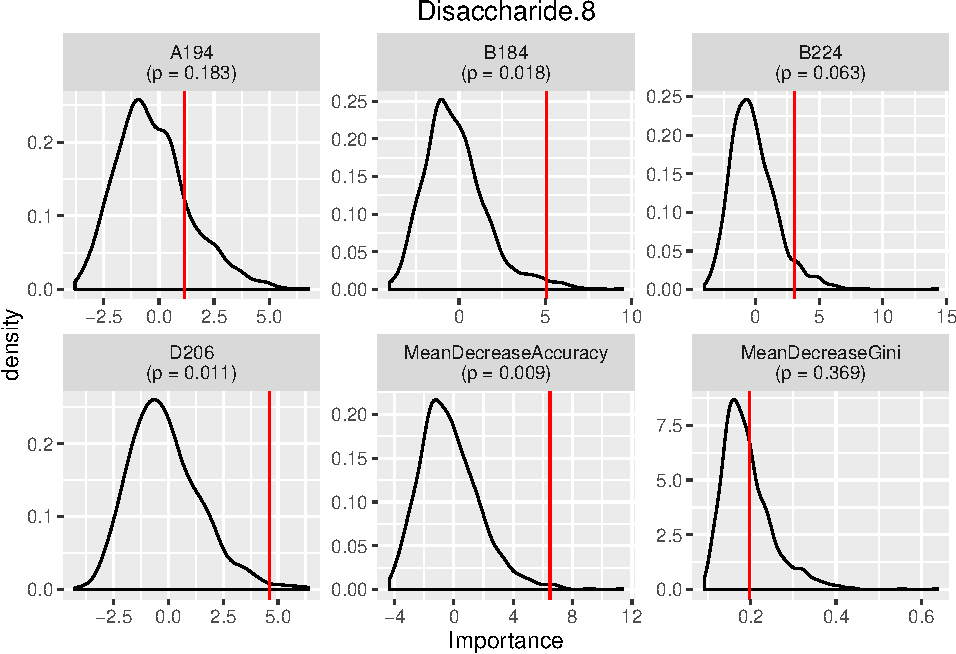
\includegraphics{archer_files/figure-latex/plotNull-1} \caption[Null distributions of importance scores for Disaccharide.8]{Null distributions of importance scores for Disaccharide.8.}\label{fig:plotNull}
\end{figure}
\end{Schunk}

It can be useful to visualize the distribution of importance scores
across all predictors and easily identify those which are significant.
In \(\CRANpkg{rfPermute}\), this is accomplished with the \texttt{plot}
function applied to the result of \texttt{rp.importance}, which produces
an ordered bar chart of all predictor importances with those significant
at a specified critical \(\alpha\) (traditionally 0.05) identifed in
red. Figure 2 shows that approximately the top half of the predictor
metabolites are deemed significant at p \textless{}= 0.05, even though
the distributon of importance scores shows a steady decline with no
obvious break in this region.

\begin{Schunk}
\begin{figure}
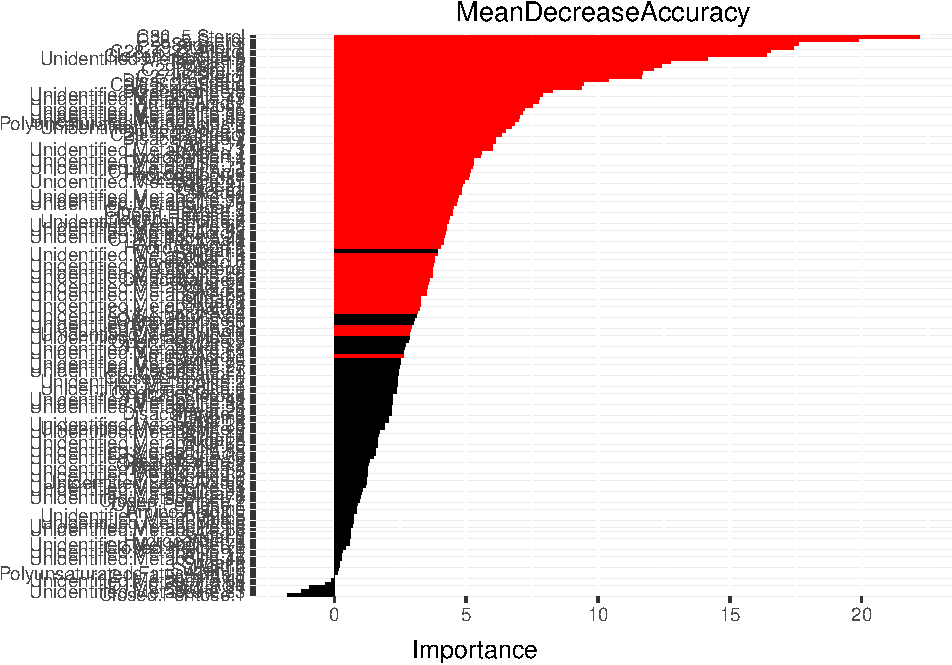
\includegraphics{archer_files/figure-latex/plot_imp1-1} \caption[Bar chart of mean decrease in accuracy]{Bar chart of mean decrease in accuracy. Bars colored in red have p-values <= 0.05.}\label{fig:plot_imp1}
\end{figure}
\end{Schunk}

Given that we can't see much detail about specific predictor metabolites
in Figure 2 due to overlap of all of the metabolite names, we can also
use the \texttt{plot} function to just show a subset, say only the top
ten most important predictors, but this time for all importance types
(Fig. 3). This figure suggests that many of the same metabolites are
significantly important for all classes. One can also restrict the
output to only significant predictors by specifyig the argument,
\texttt{sig.only\ =\ TRUE}.

\begin{Schunk}
\begin{figure}
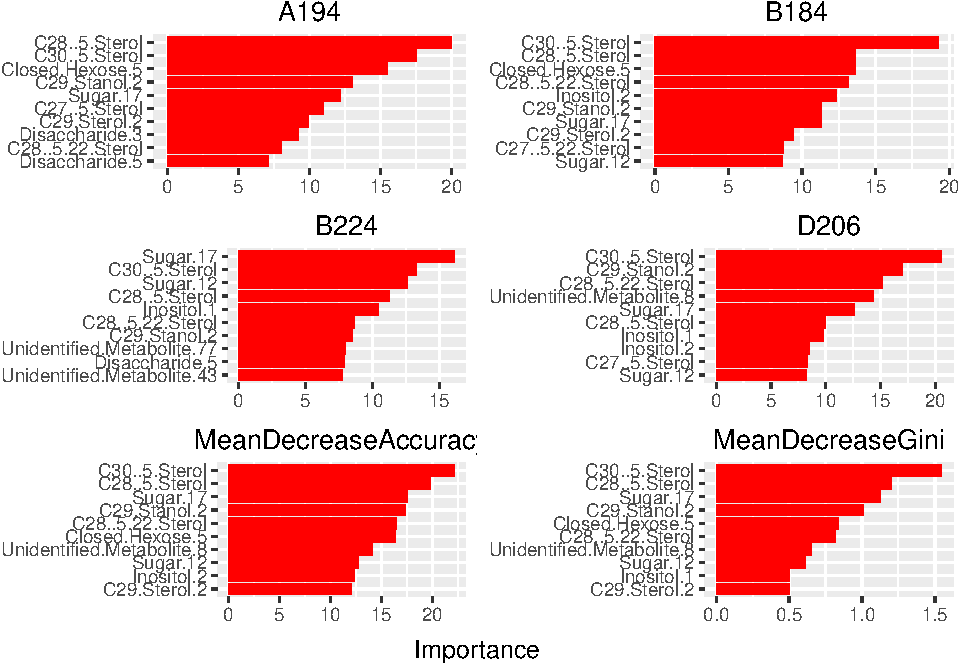
\includegraphics{archer_files/figure-latex/plot_imp2-1} \caption[Bar chart of top ten most important predictors]{Bar chart of top ten most important predictors.}\label{fig:plot_imp2}
\end{figure}
\end{Schunk}

To better visualize the relative distribution of predictor importance
across classes we can also produce a heatmap as in Figure 4 with the
\texttt{impHeatmap} function. Although many of the same metabolites rank
high for all classes, there are several lower in the list that are
significant in some classes, but not in others, suggesting that they
might have strong diagnostic properties for those subsets of classes.

\begin{Schunk}
\begin{figure}
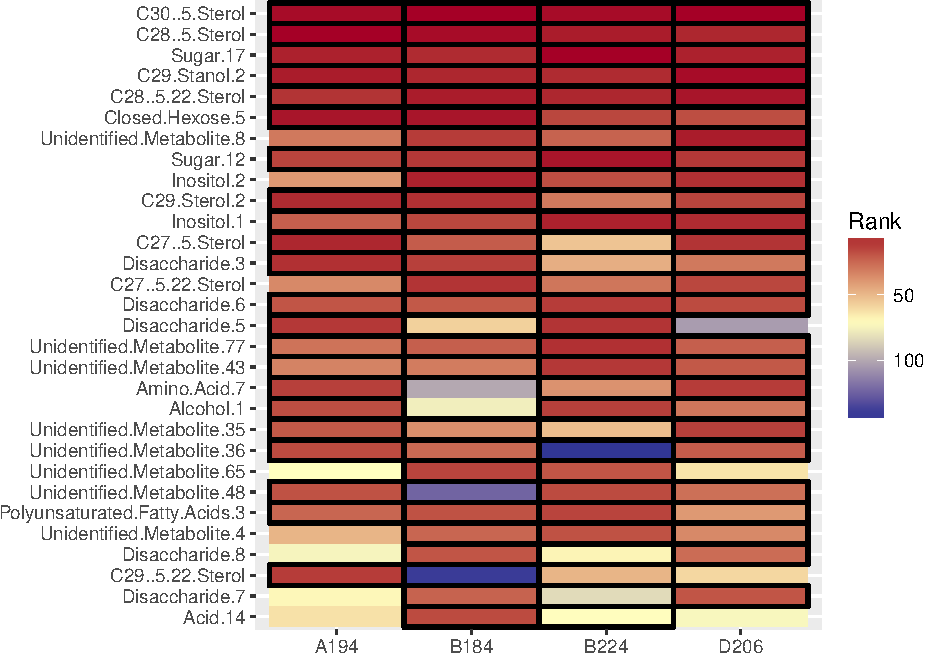
\includegraphics{archer_files/figure-latex/impHeatmap-1} \caption[Heatmap of top 30 most important predictor metabolites, color coded by rank order]{Heatmap of top 30 most important predictor metabolites, color coded by rank order. Cells encircled by black have p-values <=0.05.}\label{fig:impHeatmap}
\end{figure}
\end{Schunk}

\subsection{Model summary functions}\label{model-summary-functions}

\(\CRANpkg{rfPermute}\) also provides a set of convenient summary
functions for \(\CRANpkg{randomForest}\) models, regardless of if the
model was run in \(\CRANpkg{randomForest}\) or \(\CRANpkg{rfPermute}\).
One such function is used to evaluate how well a classification model is
performing, by calculating the OOB error rates that would expected if
samples were just randomly allocated to bins in the absence of
information from predictor variables. These rates turn out to simply be
the fraction of the total sample size represented by each class. In a
simple two-class model, with equal sample sizes in each class, this is
then 50\% for both classes. However, if the sample sizes are skewed, say
80 in class A, and 10 in class B, then one would expect on average to
correctly classify 80 / 90 of the class A samples and 10 / 90 of the
class B samples. Thus the expected error rates would be 0.11 for class A
and 0.89 for class B. These values, referred to as ``priors'' are
calculated by the \texttt{exptdErrRate} function. Since this data set
has equal sample sizes, all priors are the same:

\begin{Schunk}
\begin{Sinput}
exptdErrRate(metab.rf)
\end{Sinput}
\begin{Soutput}
 OOB A194 B184 B224 D206 
0.75 0.75 0.75 0.75 0.75 
\end{Soutput}
\end{Schunk}

The \texttt{classConfInt} function provides confidence intervals for the
class-specific and overall model classification scores based on a
binomial distribution. This helps provide a measure of uncertainty of
the true classification rate given the observed sample sizes.

\begin{Schunk}
\begin{Sinput}
classConfInt(metab.rf)
\end{Sinput}
\begin{Soutput}
        pct.correct LCI_0.95 UCI_0.95 Pr.gt_0.8
A194          0.938    0.698    0.998     0.972
B184          1.000    0.794    1.000     1.000
B224          0.938    0.698    0.998     0.972
D206          1.000    0.794    1.000     1.000
Overall       0.969    0.892    0.996     1.000
\end{Soutput}
\end{Schunk}

The first column in the output is the oberved percent correct (1 - OOB
error rate). The next two columns are the bounds of the central
95-percentile of the classification score given the observed sample
sizes. The final column provides the fraction of the binomial
distribution that is greater than a given threshold. The default is 0.8,
but it can be specified to any other value in \texttt{0:1} using the
\texttt{threshold} argument.

A complete summary of the \(\CRANpkg{randomForest}\) classification
model can be produced by combining the results of \texttt{classConfInt}
and \texttt{exptdErrRate} along with the full confusion matrix as in the
function, \texttt{confusionMatrix}.

\begin{Schunk}
\begin{Sinput}
confusionMatrix(metab.rf)
\end{Sinput}
\begin{Soutput}
        A194 B184 B224 D206 pct.correct LCI_0.95 UCI_0.95 Pr.gt_0.8 Prior
A194      15    1    0    0        93.8     69.8     99.8      97.2    25
B184       0   16    0    0       100.0     79.4    100.0     100.0    25
B224       0    0   15    1        93.8     69.8     99.8      97.2    25
D206       0    0    0   16       100.0     79.4    100.0     100.0    25
Overall   NA   NA   NA   NA        96.9     89.2     99.6     100.0    25
\end{Soutput}
\end{Schunk}

Note that in this matrix, the columns deriving from the
\texttt{classConfInt} function are multiplied by 100, and \texttt{Prior}
is 100 * (1 - expected error rate), as I have found this scale to be
more easily communicated in publications.

\subsection{Vote distributions}\label{vote-distributions}

When evaluating a Random Forest classification model, it can also be
useful to visualize the distribution of votes for classes within the
forest. From these distributions, we can tell if individual cases are
tending to be correctly classified with large probabilities (have a high
fraction of trees voting for the correct class), or have equivocal
assignments (vote probabilities are roughly equal). We can also see if
misclassified samples were strongly or weakly misclassified. The
\texttt{plotVotes} function will produce such a distribution, either as
a stacked bar chart, which is useful when few samples are present, or as
an area chart, which is more readable with many samples.

\begin{Schunk}
\begin{figure}
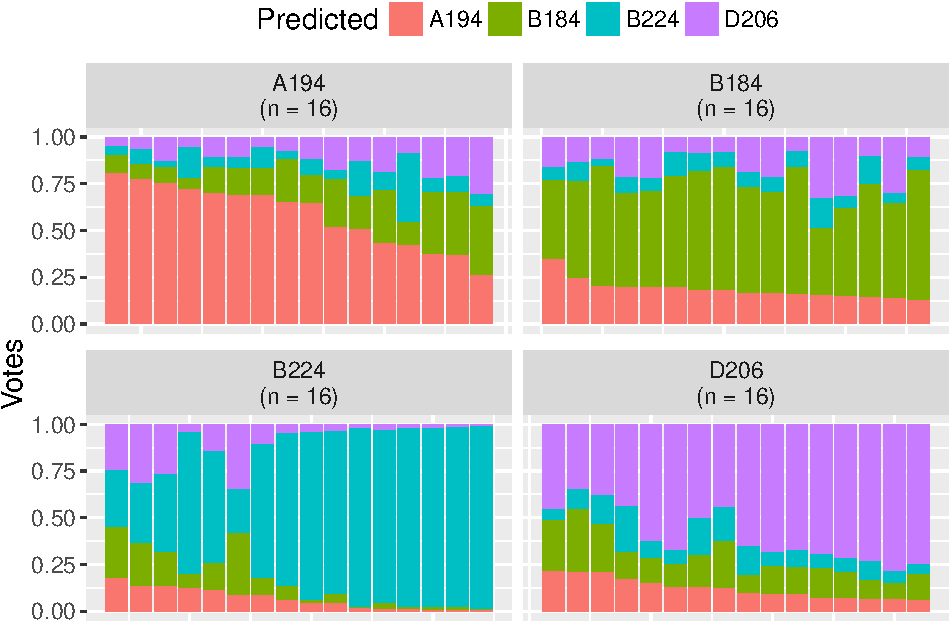
\includegraphics{archer_files/figure-latex/plotVotes-1} \caption[Distribution of votes in the Random Forest model for samples of each of the four \textit{Symbiodinium} types]{Distribution of votes in the Random Forest model for samples of each of the four \textit{Symbiodinium} types.}\label{fig:plotVotes}
\end{figure}
\end{Schunk}

Figure 5 shows that \emph{Symbiodinium} types A194 and D206 have many of
their members classified with a relatively large fraction of votes. We
also see that most of the B224 samples have a very large fraction of
trees voting for the correct species, but about a third have more votes
spread throughout other species, matching the misclassification rate for
this species.

\subsection{Proximity plots}\label{proximity-plots}

For visualizing the relative distribution of samples in the Random
Forest, multi-dimensional scaling (MDS) is applied to the proxmity
matrix computed by \texttt{randomForest}. The \(\CRANpkg{randomForest}\)
package provides the \texttt{MDSplot} function which uses \(\pkg{base}\)
graphics to visualize these points. In \(\CRANpkg{rfPermute}\) there is
the \texttt{proximityPlot} function which uses \(\CRANpkg{ggplot2}\)
graphics \citep{Wickham2009} and provides a few additional useful
features. The result of \texttt{proximityPlot} depicts the MDS
projection of cases, with classes encircled by a shaded convex hull.
Additionally, each case is represented by a color-coded dot and circle.
The color of the interior dot corresponds to the original case, while
the color of the exterior circle corresponds to the predicted case.
Thus, correctly classified cases will be composed of the same color,
while misclassified cases will have different colors.

\begin{Schunk}
\begin{figure}
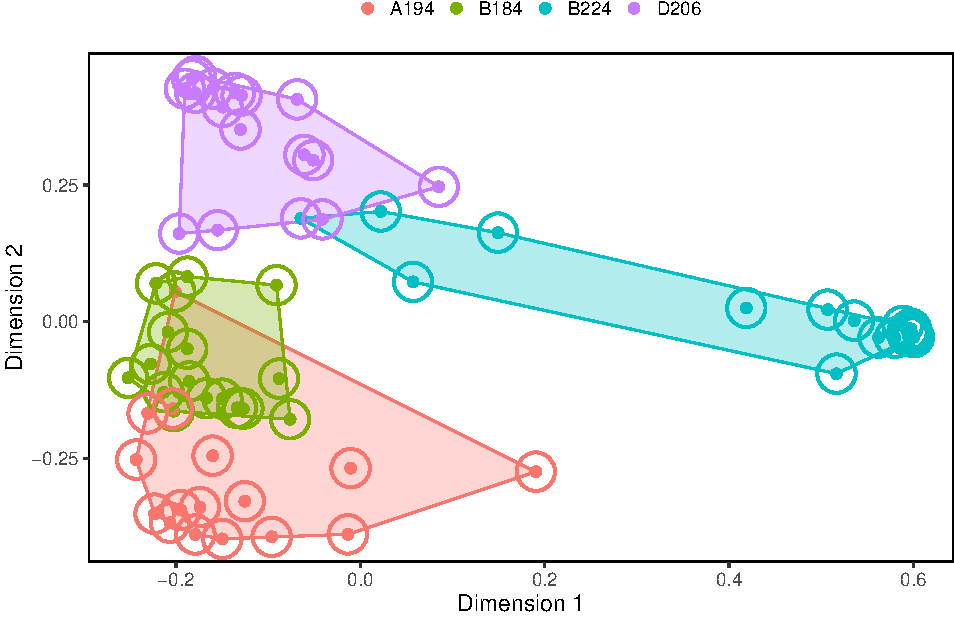
\includegraphics{archer_files/figure-latex/proximityPlot-1} \caption[Proximity plot of \textit{Symbiodinium} samples]{Proximity plot of \textit{Symbiodinium} samples.}\label{fig:proximityPlot}
\end{figure}
\end{Schunk}

In Figure 6, we can see that most of the difference in metabolite
profiles is driven by the differences between B224 and the other three
species. A194, B184, and D206 are then distributed along the second
dimension, with overlap between A194 and D206 on this dimension.
However, given that there are no misclassifications between these two
species, we suppose that they are differentiated on another dimension.
We can also see that the misclassified B224 samples are near the
periphery of the B184 and D206 convex hull, some distance away from the
majority of the other B224 samples, but also separated from the majority
of the B184 and D206 samples. This is reflected in the vote distribution
in Figure 5, and given the overall variability in B224, we might then
view these as aberrant B224 samples rather than mislabelled samples of
another species.

All graphical output in \(\CRANpkg{rfPermute}\) is produced using the
\(\CRANpkg{ggplot2}\) package. Functions that produce figures will also
invisibly return the \texttt{ggplot2} object generated so that they can
be further modified if desired. The \texttt{proximityPlot} function also
returns the MDS matrix resulting from a call to \texttt{cmdscale}.

\subsection{Performance}\label{performance}

Because the primary function, \texttt{rfPermute}, is a wrapper that
calls \texttt{randomForest} multiple times, execution time can be
lengthy for large data sets and will scale relatively linearly with the
number of permutations. However, execution time can be reduced if a
multi-core machine is used and the \texttt{num.cores} argument set
appropriately. For example, on a MacBook Pro with a 2.8GHz Intel Core i7
chip and 16GB of 1600 MHz DDR3 RAM, one \(\CRANpkg{randomForest}\) run
of the \emph{Symbiodinium} data set took approximately 0.4 seconds. The
same \(\CRANpkg{rfPermute}\) model with 100 replicates took 52 seconds,
and 1000 replicates took 537 seconds (9 minutes) on one core. When the
number of cores used was to three, the 1000 replicate model took 193
seconds (3.2 minutes).

Efficiency can also be enhanced by running the same
\(\CRANpkg{rfPermute}\) model can on multiple systems and combining the
results later using the \texttt{rp.combine} function. This function is
the equivalent of \texttt{randomForest::combine} and takes a set of the
same \(\CRANpkg{rfPermute}\) models as its arguments.

Nevertheless, with models of any size, it is advised to first run one
model with no replicates to ensure that a sufficient number of trees are
being built to produce stable OOB estimates. Stability can be verified
using the \texttt{plot} function on the model output and observing the
trace of OOB estimates for each class as well as overall.

\subsection{Installation}\label{installation}

The stable version of \(\CRANpkg{rfPermute}\) can be installed from CRAN
via:

\begin{Schunk}
\begin{Sinput}
install.packages("rfPermute")
\end{Sinput}
\end{Schunk}

To install the latest development version from GitHub, use:

\begin{Schunk}
\begin{Sinput}
# make sure you have Rtools/devtools installed
if (!require("devtools")) install.packages("devtools")

# install from GitHub
devtools::install_github("EricArcher/rfPermute")
\end{Sinput}
\end{Schunk}

\bibliography{archer}

\address{%
Frederick I. Archer\\
Southwest Fisheries Science Center\\
8901 La Jolla Shores Drive\\ La Jolla, CA 92037 USA\\
}
\href{mailto:eric.archer@noaa.gov}{\nolinkurl{eric.archer@noaa.gov}}

